\documentclass{article}
\usepackage[utf8]{inputenc}
\usepackage{amsmath}
\usepackage{natbib}
\linespread{1}
\usepackage{bm}
\usepackage{mcode}
\usepackage[lighttt]{lmodern}
\usepackage{graphicx} 
\usepackage{epstopdf}
\usepackage{algorithm2e}
\usepackage{multicol}
\usepackage{float}
\usepackage{subfigure}
\usepackage{amsmath}
\graphicspath{{figureForTex/}}
\title{\LARGE{Polymer Chain Dynamics Simulation}\\ \large{Report}
}
\author{ZHA Chenyu}
%\date{5.Mars.2015}
\renewcommand*\contentsname{Table de matière}

\begin{document}

\maketitle
\pagebreak


\section{The random walk model:the freely jointed chain}
\paragraph{}

Consider a linear polymer to be a freely-jointed chain with N beads, length of each bond is $b$ , that occupy zero volume. The path of the chains is like a 'random walk 'in three dimensions, limited only by the constraint that each segment must be joined to its neighbors.\\

Consider the 'end to end' vector $\bm{R}$ joining one end of the polymer to the other,the average value $<\bm{R}>$ is zero,since the probability of R equals -R.Therefore we will calculate $<\bm{R^2}>$
\begin{equation}
<\bm{R^2}>=\sum_{{n=1}}^{N}\sum_{m=1}^{N}<r_n\cdot r_m>
\end{equation} 
We consider that there is no correlation between bead $n$ and $m$,therefore we find :
\begin{equation}
<\bm{R^2}>=\sum_{{n=1}}^{N}<r_n^2>=Nb^2
\end{equation}
The probability distribution of $\bm{R}$ is:
\begin{equation}
P(\bm{R},N)=(\frac{3}{2\pi Nb^2})^{3/2}exp(-\frac{3\bm{R}^2}{2Nb^2})
\end{equation}
The probability distribution function of $\bm{R}$ obeys the Gaussian distribution.
The position of the beads after each step will satisfy the diffusion equation :
\begin{equation}
\bm{R(t+\Delta t)}=\bm{R(t)}+\sqrt{2D\Delta t}\bm{g(t)}
\end{equation}
$\bm{g(t)}$ is normally distributed random noise.
\subsection{Random walk Simulation}
We simulate the random walk with the following parameters :
\begin{lstlisting}
dimension      = 3;;%dimension=1,2 or 3
numParticles   = 100;%number of particles in polymers;
dt             =0.1;%pas de temps
numSteps       =100;% number of motion
diffusionConst =0.1; %constante diffusion
paths          =[];  ; %the paths of polymer;
\end{lstlisting}
The following graph is the trajectory of beads in the first step and last step;
\begin{figure}[H]
	\begin{minipage}[t]{0.5\textwidth}
		\centering
	
		
		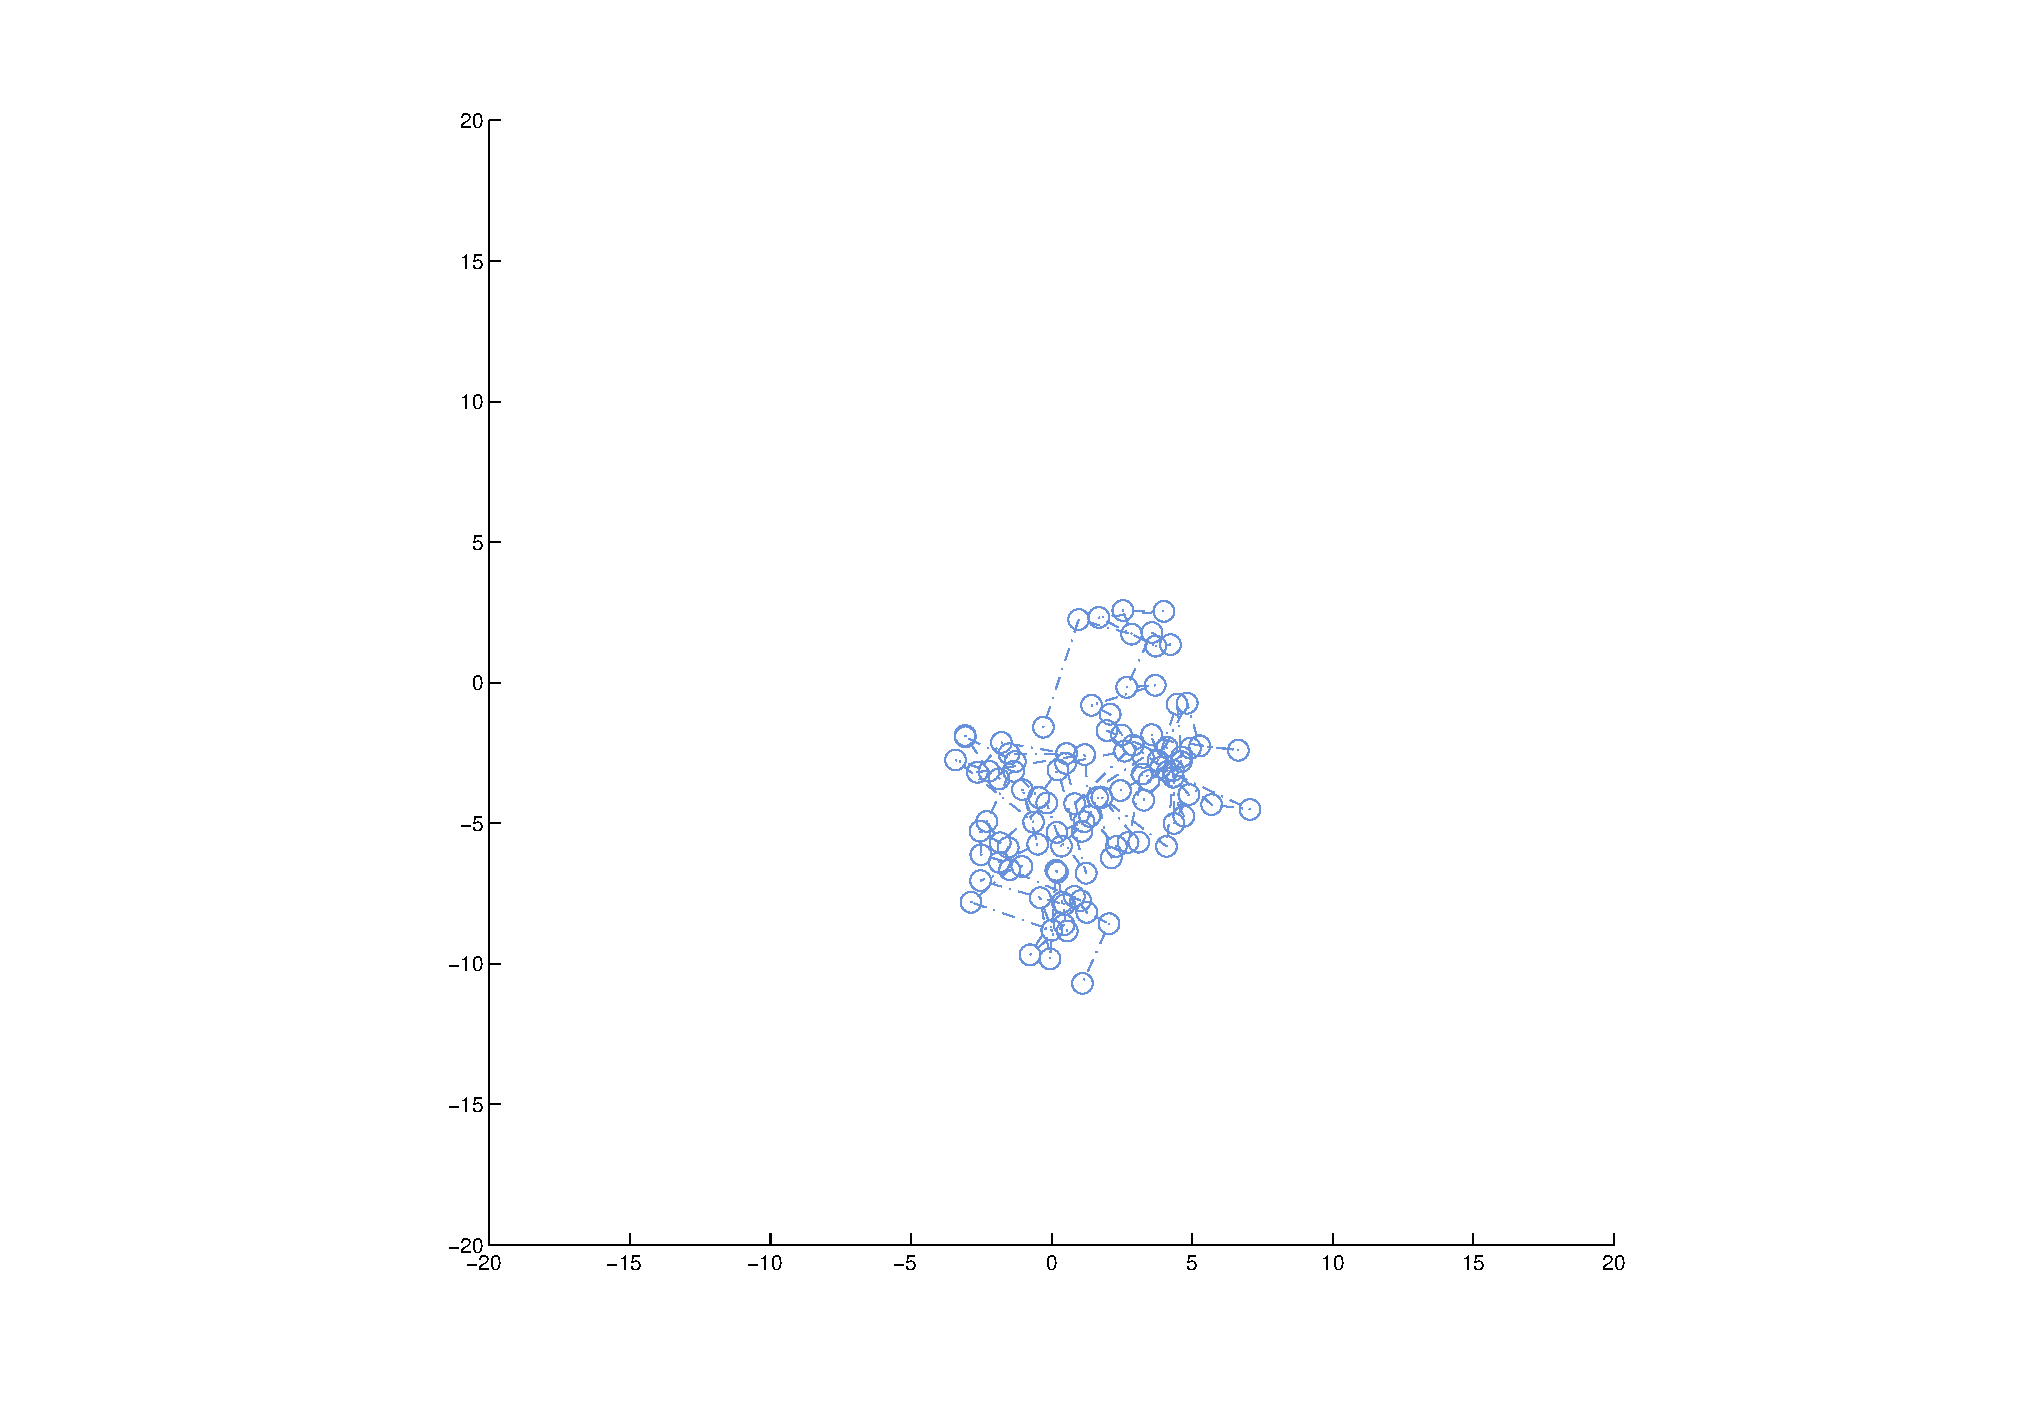
\includegraphics[width=3.2in]{1.eps}
		\caption{initial position}
	\end{minipage}%
	\begin{minipage}[t]{0.5\textwidth}
		\centering
		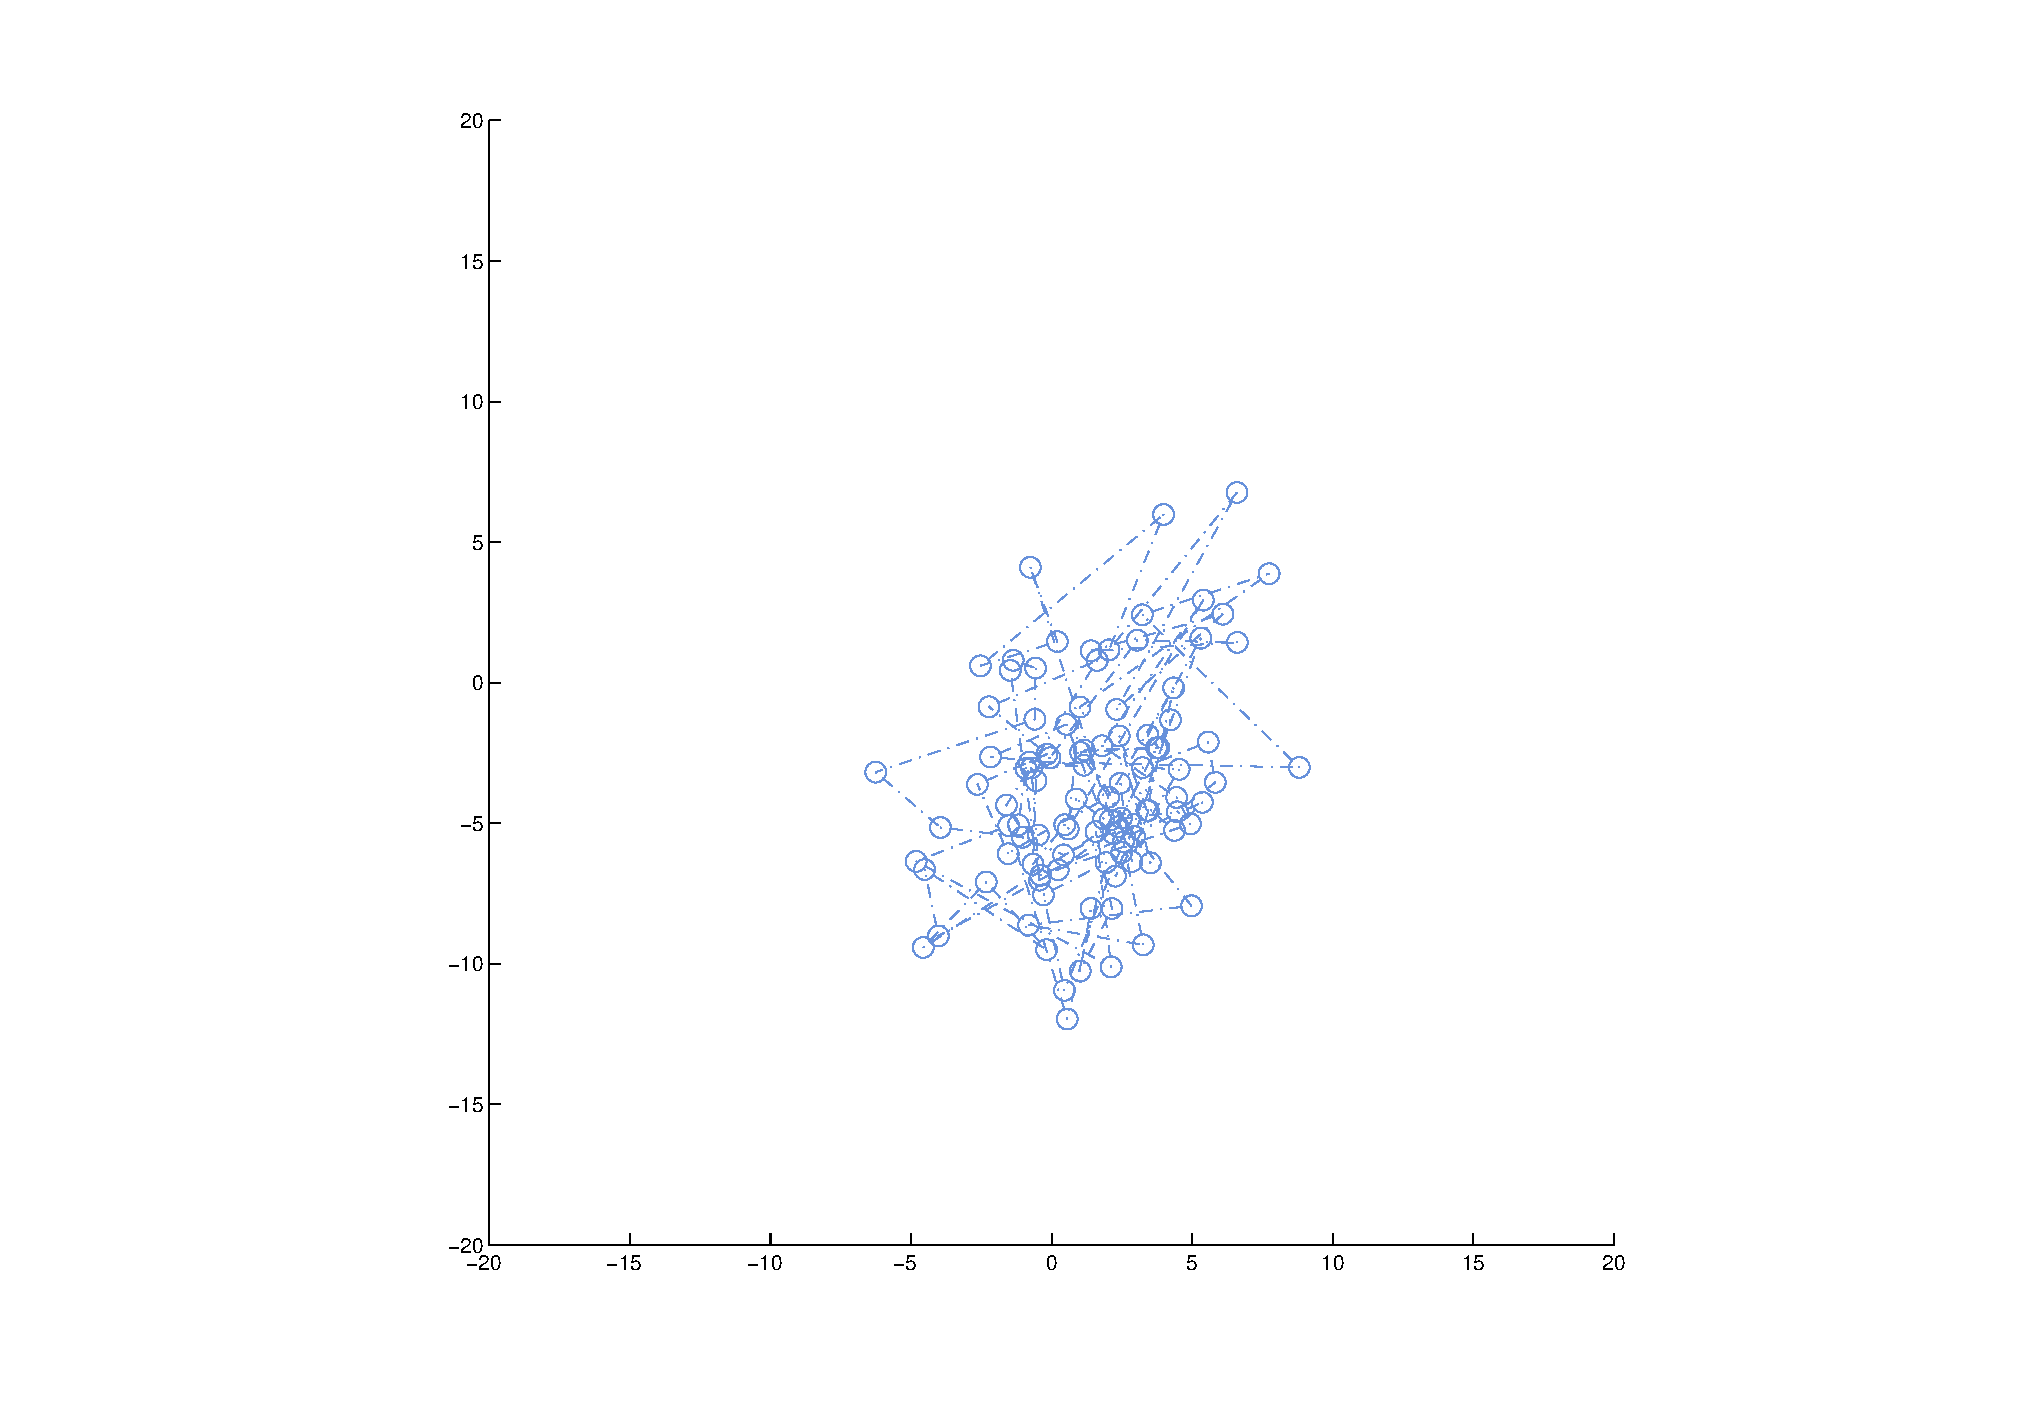
\includegraphics[width=3.2in]{2.eps}
		\caption{final position}
		
	\end{minipage}
\end{figure}
\subsection{Probability density function of $\bm{R}$ }
In order to verify that the PDF of $\bm{R}$ is Gaussian,we calculate the 'end to end distance' $\bm{R}$ for each simulation,then we plot it with histogram by coordinate $(x,y,z)$ respectively and compare with the probability density function of $\bm{R}$ in theory. \\
We simulate the probability density of Gaussian  with the following parameters :
\begin{lstlisting}

     dimension: 3
     numParticles: 100
     dt: 0.1000
     numSteps: 100
     diffusionConst: 0.1000
     paths: [2x3x2 double]
     simulation: 1000

\end{lstlisting}
The following graphs verify that for each coordinate,the distribution of $\bm{R}$ is Gaussian;
\begin{figure}[H]
	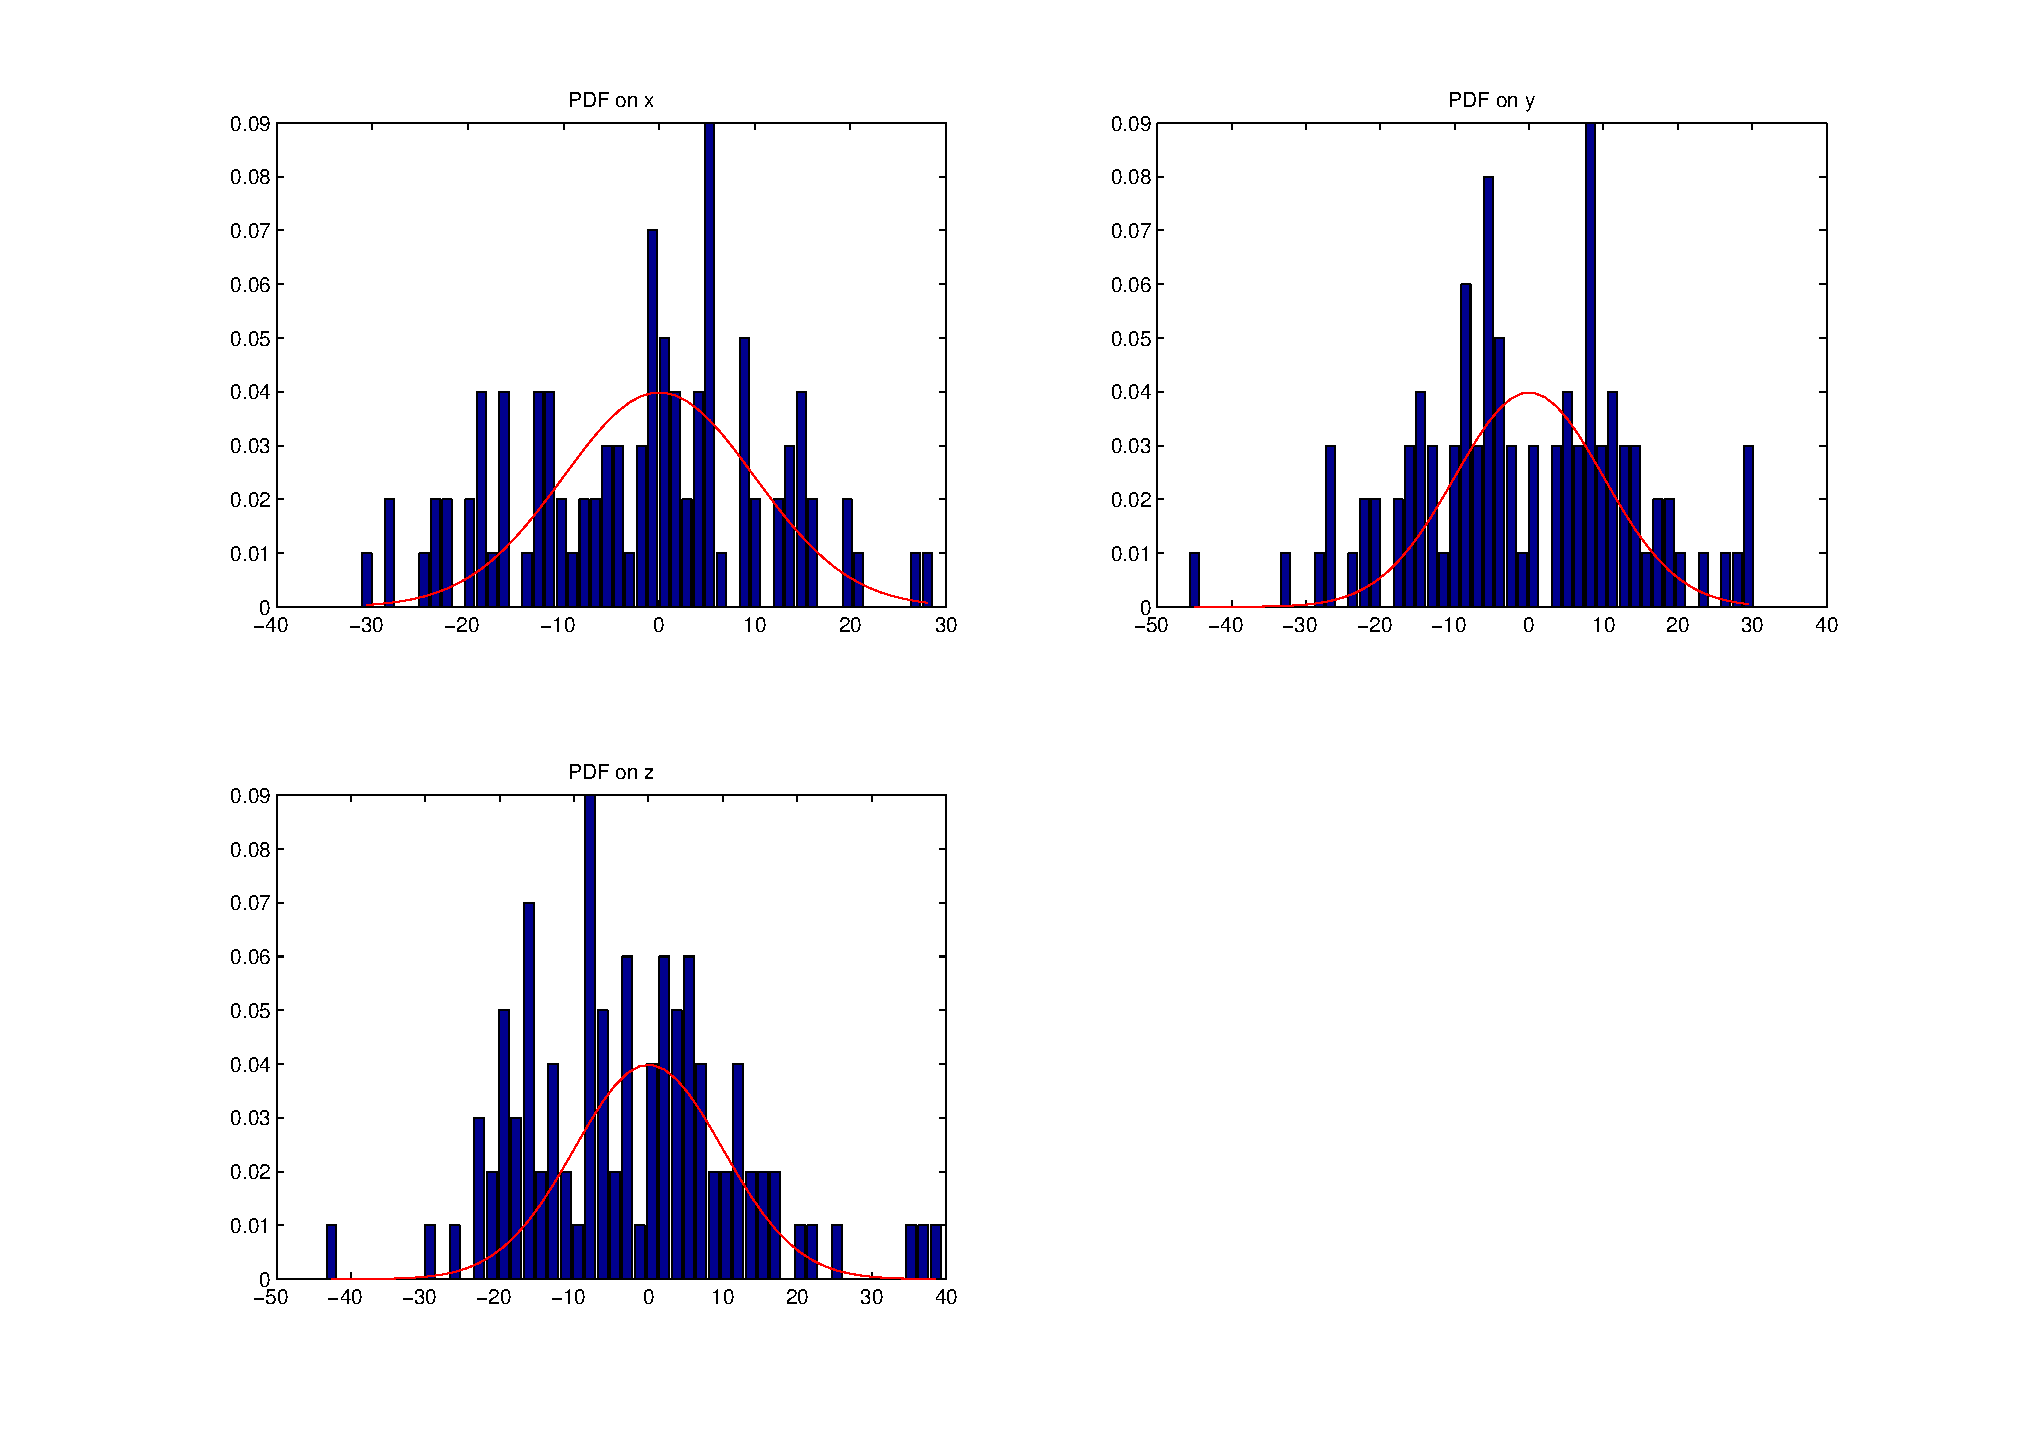
\includegraphics[width=6.2in]{PDF.eps} 
	 
	 \end{figure}
	 \section{The bead-spring model}
	 \paragraph{}
	 The bead-spring model is also called Rouse Model .In this model,the single chain diffusion is represented by Brownian motion ,there is no exclude volume 	interactions between the beads and each bead experience a drag force proportional to their velocity ,then the position of the beads will satisfy the Langevin equation :
	 \begin{equation}
	 \frac{d\bm{R_n}}{dt}=\frac{k}{\xi}(\bm{R_{n+1}}+\bm{R_{n-1}}-2\bm{R_{n}})+\bm{g_n}, \forall n \in [1,2...N-1]
	 \end{equation}
	 For the bead $0$ and $N$,we have :
	 \[
	 \begin{cases}
	\frac{d\bm{R_0}}{dt}=\frac{k}{\xi}(\bm{R_{1}}-\bm{R_{0}})+\bm{g_n}\\
	\frac{d\bm{R_n}}{dt}=\frac{k}{\xi}(\bm{R_{n-1}}-\bm{R_{n}})+\bm{g_n}
	 \end{cases}
	 \]
	 where $\xi$ is friction coefficient,$k$ is spring constant.
	 \subsection{Rouse Model Simulation}
	 We simulate the Rouse Model with the following parameters:
	 \begin{lstlisting}
	  dimension: 3
	  numParticles: 100
	  dt: 0.1000
	  numSteps: 100
	  diffusionConst: 0.1000
	  paths: [100x3x100 double]
	  simulation: 1
	  pathsNormal: [100x3x100 double]
	  frictionCoefficient: 1
	  connectedBeads: []
	  fixedBeads: []
	  b: 1
	 \end{lstlisting}
	 The following graph is the trajectory of beads in the first step and last step;
	 \begin{figure}[H]
	 	\begin{minipage}[t]{0.5\textwidth}
	 		\centering
	 		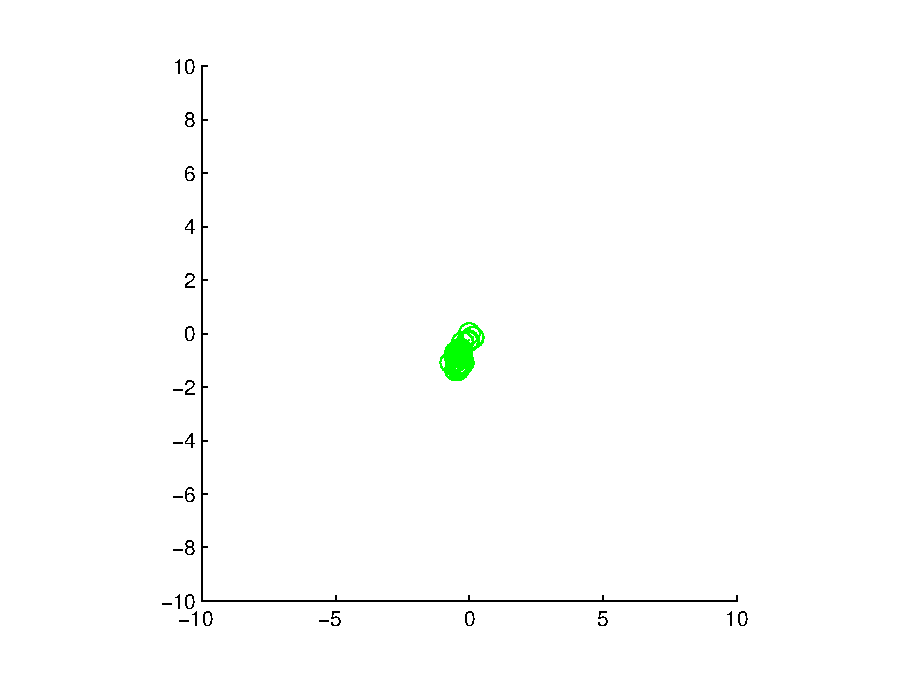
\includegraphics[width=3.2in]{rouseM.eps}
	 		\caption{initial position}
	 	\end{minipage}%
	 	\begin{minipage}[t]{0.5\textwidth}
	 		\centering
	 		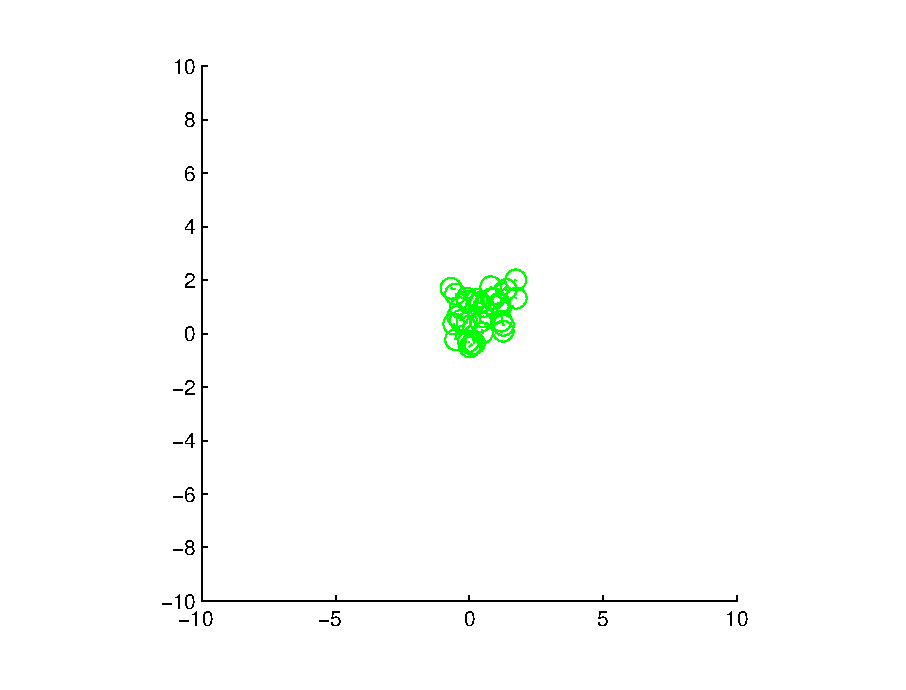
\includegraphics[width=3.2in]{rouseMF.eps}
	 		\caption{final position}
	 		
	 	\end{minipage}
	 \end{figure}
\subsection{Simulation of the mean first-encounter time in the Rouse Model}
\paragraph{}
We want to simulate the mean first-encounter time that 3 beads have met each other in a chain during each simulation, in order to verify that the probability distribution function is exponential.We set 32 beads and we do the simulations with the first bead,last bead ,the third bead we set it from 2 to 16,because it's symmetric.that means we have $[1,2,32],[1,3,32]...[1,16,32]$ cases.For each case,we calculate the mean first-encounter time and we plot with histogram.
\begin{figure}[H]
	\includegraphics[width=4.2in]{intro.jpg}
	\caption{$k\in [1,31]$ }
\end{figure}

At first,we compare the mean encounter time between 2 beads and 3 beads with the following parameters:
\begin{lstlisting}
dimension           = 3;
numParticles        = 32;
dt                  = 0.01;
diffusionConst      = 10;
numSteps            = Inf;
numSimulations      = 1000;
frictionCoefficient = 1;
connectedBeads      = [];
fixedBeads          = [];
metBeadNum          = [1 16 32] [1 32];
b                   = 1;
encounterDistance   = 3*b./5;
encounterTime       a list contains the time they have met for every simulation;      
\end{lstlisting}
\begin{figure}[H]
	\centering
	\includegraphics[width=6.2in]{2beads_3beads.eps}
	\caption{The first encounter time of [1 16 32] and [1 32]}
\end{figure}
\pagebreak
We compare also the first encounter time with beads from [1 2 32] to [1 16 32]:\\
\begin{lstlisting}
dimension           = 3;
numParticles        = 32;
dt                  = 0.01;
diffusionConst      = 10;
numSteps            = Inf;
numSimulations      = 1000;
frictionCoefficient = 1;
connectedBeads      = [];
fixedBeads          = [];
metBeadNum          = [1 2 32].. [1 16 32];
b                   = 1;
encounterDistance   = 3*b./5;
encounterTime       a list contains the time they have met for every simulation;      
\end{lstlisting}
\begin{figure}[H]
	\begin{minipage}[t]{0.5\textwidth}
		\centering
		\includegraphics[width=3.2in]{beads1_2_32.eps}
		\end{minipage}%
		\begin{minipage}[t]{1.0\textwidth}
			\centering
			\includegraphics[width=3.2in]{encounterBeads1_2_32.jpg}
			\end{minipage}
			\caption{[1 2 32]}
		\end{figure}
		\begin{figure}[H]
			\begin{minipage}[t]{0.5\textwidth}
				\centering
				\includegraphics[width=3.2in]{beads1_3_32.eps}
			\end{minipage}%
			\begin{minipage}[t]{1.0\textwidth}
				\centering
				\includegraphics[width=3.2in]{encounterBeads1_3_32.jpg}
			\end{minipage}
		    \caption{[1 3 32]}
		\end{figure}
			\begin{figure}[H]
				\begin{minipage}[t]{0.5\textwidth}
					\centering
					\includegraphics[width=3.2in]{beads1_4_32.eps}
				\end{minipage}%
				\begin{minipage}[t]{1.0\textwidth}
					\centering
					\includegraphics[width=3.2in]{encounterBeads1_4_32.jpg}
				\end{minipage}
			    \caption{[1 4 32]}
			\end{figure}
				\begin{figure}[H]
					\begin{minipage}[t]{0.5\textwidth}
						\centering
						\includegraphics[width=3.2in]{beads1_5_32.eps}
					\end{minipage}%
					\begin{minipage}[t]{1.0\textwidth}
						\centering
						\includegraphics[width=3.2in]{encounterBeads1_5_32.jpg}						
					\end{minipage}
					\caption{[1 5 32]}
				\end{figure}
					\begin{figure}[H]
						\begin{minipage}[t]{0.5\textwidth}
							\centering
							\includegraphics[width=3.2in]{beads1_6_32.eps}
						\end{minipage}%
						\begin{minipage}[t]{1.0\textwidth}
							\centering
							\includegraphics[width=3.2in]{encounterBeads1_6_32.jpg}
						\end{minipage}
						\caption{[1 6 32]}
					\end{figure}
						\begin{figure}[H]
							\begin{minipage}[t]{0.5\textwidth}
								\centering
							\includegraphics[width=3.2in]{beads1_7_32.eps}
							\end{minipage}%
							\begin{minipage}[t]{1.0\textwidth}
								\centering
							\includegraphics[width=3.2in]{encounterBeads1_7_32.jpg}
							\end{minipage}
							\caption{[1 7 32]}
						\end{figure}
							\begin{figure}[H]
								\begin{minipage}[t]{0.5\textwidth}
									\centering
							\includegraphics[width=3.2in]{beads1_8_32.eps}
								\end{minipage}%
								\begin{minipage}[t]{1.0\textwidth}
									\centering
							\includegraphics[width=3.2in]{encounterBeads1_8_32.jpg}
								
								\end{minipage}
									\caption{[1 8 32]}
							\end{figure}
                            \begin{figure}[H]
                            \begin{minipage}[t]{0.5\textwidth}
                            	\centering
                            	\includegraphics[width=3.2in]{beads1_16_32.eps}
                            \end{minipage}%
                            \begin{minipage}[t]{1.0\textwidth}
                            	\centering
                            	\includegraphics[width=3.2in]{encounterBeads1_16_32.jpg}
                            	
                            \end{minipage}
                            \caption{[1 16 32]}
                            \end{figure}						
For each pair of beads,we calculate the mean first-encounter time:
\begin{figure}[H]
\centering
\includegraphics[width=5in]{beads32meanEncounterTime.eps}
\end{figure}
\pagebreak
To verify that it's symmetric,we calculate the mean first-encounter time for all the beads with 10000 simulations for each pair :\\
\begin{figure}[H]
\includegraphics[width=6in]{beads32meanEncounterTimeAll.eps}
\end{figure}
\begin{lstlisting}
dimension           = 3;
numParticles        = 32;
dt                  = 0.01;
diffusionConst      = 10;
numSteps            = Inf;
numSimulations      = 10000;
frictionCoefficient = 1;
connectedBeads      = [];
fixedBeads          = [];
metBeadNum          = [1 2 32].. [1 31 32];
b                   = 1;
encounterDistance   = 3*b./5;
encounterTime       a list contains the time they have met for every simulation;      
\end{lstlisting}
\pagebreak
Then we change the number of beads to 64,we simulate the first encounter time with the same parameters and we set the $metBeadNum$ from[1 2 64] to [1 11 64] :\\
\begin{lstlisting}
dimension           = 3;
numParticles        = 64;
dt                  = 0.01;
diffusionConst      = 10;
numSteps            = Inf;
numSimulations      = 1000;
frictionCoefficient = 1;
connectedBeads      = [];
fixedBeads          = [];
metBeadNum          = [1 2 64].. [1 31 64];
b                   = 1;
encounterDistance   = 3*b./5;
encounterTime       a list contains the time they have met for every simulation;      
\end{lstlisting}
We compare the mean first-encounter time between 32 and 64 beads :\\
	\begin{figure}[H]
		\begin{minipage}[t]{0.5\textwidth}
			\centering
			\includegraphics[width=3.2in]{compare1_2_64and1_2_32.eps}
			
		\end{minipage}%
		\begin{minipage}[t]{1.0\textwidth}
			\centering
			\includegraphics[width=3.2in]{compare1_3_64and1_3_32.eps}
			
		\end{minipage}
	\end{figure}
	\begin{figure}[H]
		\begin{minipage}[t]{0.5\textwidth}
			\centering
			\includegraphics[width=3.2in]{compare1_4_64and1_4_32.eps}
			
		\end{minipage}%
		\begin{minipage}[t]{1.0\textwidth}
			\centering
			\includegraphics[width=3.2in]{compare1_5_64and1_5_32.eps}
		
		\end{minipage}
	\end{figure}	
According the results,we can assume that with the number of beads increase twice,the mean first-encounter time takes 4 times longer ;  					
\begin{figure}[H]
	\centering
	\includegraphics[width=6.5in]{meanEncounterTimeCompareBis.eps}
\end{figure}
\section{Chains simulations in domains}
\paragraph{}
The simulation with several chains in domains are used to  
simulate the motion of yeast's chromosomes. The centromeres (middle 
point) of the chromosomes are anchored to the nucleus membrane,
and the telomeres (end points) are either diffusion on the membrane 
or are detached and diffuse inside the nucleus.The telomeres can be also sticked(connected) and disconnected between them.\\
\begin{figure}[H]
	\centering
	\includegraphics[width=5in]{chainsFixedBeads.jpg}	
\end{figure}
\subsection{Define domain and chains}
\paragraph{}
A domain is defined by the class $DomainHandler$ which contains \\
properties(ex:domainShape,dt)to build up the domain,in addition,some \\
forces associated (ex:springForce,diffusionForce) which is in the\\ class $ForceManageParams$.\\

The class $ObjectManager$ manages all objects located within the domain of the $simulationFramework$ class. A chain is defined by class $ChainParams$ 
below $ObjectManager$ and which should also have some forces associated located in the class $ForceManageParams$.\\	
The mainly structure of Rouse chains simulation is :\\
\begin{figure}[H]
	\includegraphics[width=6.6in]{structure.jpg}
\end{figure}
\subsection{Attachment and Detachment on the boundary}
\paragraph{}
To attach and detach the telomeres from the nucleus membrane,
the procedure will be broken down with mainly 4 steps :\\

1.Define severals chains in the domain.For the beads inside the domain, do 

the random walk ,for the beads on the boundary ,

diffuse them on the boundary(sphere);\\

2.For each chain ,imported fixed points on surface;\\

3.Clustering of points on the boundary(create Brownian bridge);\\

4.Attachment/detachment from boundary;

\subsubsection{Brownian bridge}
The Brownian bridge is a Brownian motion which is starting at $x$ at time $t_0$ and passing through point $y$ at $T$, $T \geq t$,it is defined as :\\
\begin{equation}
B(t) = w(t-t_0)-\frac{t-t_0}{T-t_0}[w(T-t_0)-y+x]+x
\end{equation}
which $w(T)$ is a random walk process.\\
The following steps are used to build a Brownian bridge in domain :\\

1.Initialization of beads on the domain's boundary;\\

2.List all constrain beads in ascending order $c={a_1,a_2,...a_{N_c}}$\\

3.Choose a random position for $B_{a_1}$;\\

4.For $i =2...N_c$,choose a position for $B_{a_i}$ by diffusion on the boundary $a_i -a_{i-1}$ steps;\\

5.For all of points in $c$,if $a_{i}-a_{i-1}>1$,construct a Brownian bridge between each 2 points by using the formula above;\\

6.If $a_1 \geq 1$ or $a_{N_c} \leq BeadsEnd,$sequentially build a path form the 1 to $a_1$ and $a_{N_c}$ to $BeadsEnd$.\\

The following parameters and functions are used to simulate :\\

Parameters :
\begin{lstlisting}
domainNum         = 1;
dimension         = 3;
domainShape       = 'sphere';
domainWidth       = 2;
domainCenter      = [0 0 0];
showDomain        = true;
dt                = 0.01;
diffusionConst    = 1;
numBeads          = 100;
domainClass       = domainHandler;
beads             = [15 50 90];% beads on the boundary
\end{lstlisting}

Functions :
\begin{lstlisting}
chainPath = BrownianBridgeSim(initialPoint,domainClass,domainNum,beadsOnBoundary,numBeads)
points    = BeadsOnBoundary(initialPoint,radius,domainCenter, dt, diffusionConst,beadIndices)
paths     = DiffusionOnSphere(initialPoint,dt,diffConst,numSteps,domainCenter,radius)
\end{lstlisting}
\begin{figure}[H]
\includegraphics[width=4.2in]{3func.jpg}
\end{figure}
\paragraph{Diffusion On Sphere}
\paragraph{}
To diffuse a path on the sphere, we do with the following steps :\\

1.generate a path in 2D;\\

2.Set a initial point which is on the sphere ,find the angles $\phi$ and $\theta$\\ 

in the spherical coordinates;\\

3.Rotate the path to the initial Point;\\

4.Project the path back on sphere;\\
\begin{figure}[H]
\includegraphics[width=3in]{diffuseOnSphere.jpg}	
\end{figure}
To generate a path 2D, we use the diffusion equation :\\
\begin{equation}
R(t+\Delta t) = R(t)+\sqrt{2Ddt}g(t)
\end{equation}
where R is 'end to end' vector with the position of N beads,$D$ is diffusion constant ,$g(t)$ is noise with Gaussian distribution;\\

With initial point$(x,y,z)$ ,calculate the angles $\theta$ and $\phi$ on sphere:\\
\[
\theta=\arctan{\frac{y}{x}}
\]
\[
\phi  =\arctan{\frac{\sqrt{x^2+y^2}}{z}}
\]

Define the rotate matrix A:\\
\begin{equation}
A = Az*Ay*Ax;
\end{equation}

$Ax =$
$\begin{pmatrix}1&0&0\\ 
	0&cos(-\phi)&sin(-\phi)\\ 
	0&-sin(-\phi)&cos(-\phi)\\ 
\end{pmatrix}$ ,
$Ay=$
$\begin{pmatrix}cos(-\phi)&0&-sin(-\phi)\\ 
0&1&0\\ 
sin(-\phi)&0&cos(-\phi)\\ 
\end{pmatrix}$

$Az=$
$\begin{pmatrix} 
cos(\theta)&sin(\theta)&0\\
-sin(\theta)&cos(\theta)&0\\ 
0&0&1\\ 
\end{pmatrix}$

Then rotate the path such that the initial point becomes the first point on the path :\\
\[
R_{rotate} = r+A*R
\]
where $r$ is the radius of sphere;\\

In order to project back on sphere ,calculate the distance between each point $P(i)$ on the path and the domain center $P_c$:\\
\[
L(i)=\sqrt{(P_x(i)-P_{cx})^2+(P_y(i)-P_{cy})^2+(P_z(i)-P_{cz})^2}
\]
Calculate the slope to find the intersection points $pI(i)$(points on sphere):\\
\[
k(i)=L(i)/r;
\]
\begin{equation}
\begin{cases}
pI_x(i)=p_{cx}+(P_x(i)-p_{cx})k(i)\\
pI_y(i)=p_{cy}+(P_y(i)-p_{cy})k(i)\\
pI_z(i)=p_{cz}+(P_z(i)-p_{cz})k(i)
\end{cases}
\end{equation}

The following graph describes how to project a path back on sphere :\\
\begin{figure}[H]
	\includegraphics[width=6.5in]{pathAfterProject.eps}
\end{figure}
\paragraph{Beads on boundary}
\paragraph{}
1.Use the function $DiffusionOnSphere$ to get the path of beads on the

 boundary;\\

2.Pick up the positions of beads which match the index of the beads on the 

boundary that initialize;\\


$DiffusionOnSphere \Longrightarrow $
$\begin{cases}
path from 15 to 50 \\ path from 50 to 90
\end{cases} \Longrightarrow BeadsOnboundary$
$\begin{cases}
position [15,50]\\
position [50,90]\\
\end{cases}$

\pagebreak
\paragraph{Brownian Bridge Simulation}
\paragraph{}
Then we simulate for 100 beads,with beads [15 50 90] on the boundary :\\
\begin{figure}[H]
\centering
\includegraphics[width=6in]{bOnB1.eps}	
\end{figure}
\paragraph{Simulations of attachment on the boundary}
\paragraph{}
The following figures represent the motion of 2 chains with the 

parameters below :\\
 \begin{lstlisting}
 chainForce : 'springForce'
              'diffusionForce'
              'diffusionConst'    = 0.1
               'springConst'      = 1
              
              
 chain(1)  : 'numBeads'            = 64 
             'lengthBeads'         = sqrt(3)
             'fixedBeadNum'        = 32
             'fixedBeadsPosition'  = initialPt
             'beadsOnBoundary'     =[1 64]
             'dt'                  = 0.1
             'chainForce'
             
 chain(2)  : 'numBeads'            = 64 
             'lengthBeads'         = sqrt(3) 
             'fixedBeadNum'        = 32
             'fixedBeadsPosition'  = initialPt
             'beadsOnBoundary'     =[1 64]
             'dt'                  = 0.1
             'chainForce'
 \end{lstlisting}
\begin{figure}[H]
	\begin{minipage}[t]{0.55\textwidth}
		\centering
		\includegraphics[width=3.2in]{step335.jpg}	
		\caption{Time=33.5s}
	\end{minipage}%
	\begin{minipage}[t]{1.0\textwidth}
		\centering
		\includegraphics[width=3.2in]{step1359.jpg}
	    \caption{Time=135.9s}
	\end{minipage}
\end{figure}
\pagebreak
With the same parameters,we can also let the intersection bead moved 
on the boundary :\\
\begin{figure}[H]
	\begin{minipage}[t]{0.55\textwidth}
		\centering
		\includegraphics[width=3.2in]{step316.jpg}	
		\caption{Time=61.8s}
	\end{minipage}%
	\begin{minipage}[t]{1.0\textwidth}
		\centering
		\includegraphics[width=3.2in]{step4090.jpg}
		\caption{Time=556.5s}
	\end{minipage}
\end{figure}
\subsubsection{Detachment from boundary }
The function $DetachmentFromBoundary$ is used to detach the last index of beads from boundary ,once the beads are detached , il move randomly in domain .
The detachment is done with following steps :\\

1.calculate the vector between the domain center and the bead chosen 

to detach ;\\

2.Reset the position by multiply the vector with a number between [0,1];\\

3.Deal the current and previous position to the objects and their members.\\
\paragraph{Simulation of detachment on the boundary}
\paragraph{}
 With the same parameters above ,we simulate the detachment of the end bead
 
 of each chain  after 2000 steps(200s):\\
\begin{figure}[H]
	\begin{minipage}[t]{0.5\textwidth}
		\centering
		\includegraphics[width=3.2in]{step1499.jpg}	
		\caption{Attachment(Time=149.9s)}
	\end{minipage}%
	\begin{minipage}[t]{1.1\textwidth}
		\centering
		\includegraphics[width=3.2in]{step7634.jpg}
		\caption{Detachment(Time=763.4s)}
	\end{minipage}
\end{figure}
\subsection{Sticky beads in domain}
\paragraph{}
As we have defined several chains in domain with first and last bead moving on the boundary ,those beads could be sticked between the chains if they get close or disconnected with some probability.\\

We are interested to simulate number of clusters en average after they have sticked and how long does it takes to form the clusters.  
\end{document}